\documentclass[a4paper]{iacas}

\usepackage{cite}
\usepackage{hyperref}% embedding hyperlinks [must be loaded after dropping]
\usepackage{amsmath,amsthm,amssymb,amsfonts,latexsym,mathrsfs,wasysym}
\usepackage{marvosym}
\usepackage{subcaption}
\usepackage{soul,color}
\usepackage{threeparttable}% tables with footnotes
\usepackage{dcolumn}% decimal-aligned tabular math columns
\usepackage{float}
\usepackage{graphicx}
\usepackage{accents}
\usepackage{tikz}
\usepackage{lastpage}
\usepackage{fancyhdr}
\usepackage{color}
\usepackage{cancel}
\usepackage{setspace}
\usepackage{enumitem}
%\doublespacing
% or:
\onehalfspacing
%\usepackage[T1]{fontenc}
%\usepackage{bigfoot} % to allow verbatim in footnote
\usepackage[framed,numbered]{matlab-prettifier}
\pagestyle{plain}
%\usepackage[hebrew,english]{babel}
\usetikzlibrary{shapes.geometric, arrows, calc}

\newcolumntype{d}{D{.}{.}{-1}}
\graphicspath{{figures/}}

% define some commands to maintain consistency
\newcommand{\pkg}[1]{\texttt{#1}}
\newcommand{\cls}[1]{\textsf{#1}}
\newcommand{\file}[1]{\texttt{#1}}
\newcommand{\sgn}[1]{\operatorname{sgn}\left(#1\right)}
\newcommand{\sat}[1]{\operatorname{sat}\left(#1\right)}
\newcommand{\rrule}[1]{\rule[#1]{0pt}{0pt}}
\newcommand{\fracds}[2]{\frac{\displaystyle #1\rrule{-0.2em}}{\displaystyle #2\rrule{1em}}}
\newcommand{\figref}[1]{Fig.~\ref{#1}}
\newcommand{\ubar}[1]{\underaccent{\bar}{#1}}
\newcommand{\norm}[1]{\lvert \lvert \vec #1 \rvert \rvert}

%diffeomorphism

\begin{document}

\begin{center}
 \large Algorithms and Application in Computer Vision - 046746
 \end{center}
\begin{center}
\large\textbf{Homework \#2}
 \end{center}


\begin{tabular}{l}
\\
{\bf\textit{Alexander Shender 328626114}} \\
{\bf\textit{Vladimir Tchuiev 309206795}} \\
Technion - Israel Institute of Technology
\end{tabular}


\newpage

\section{Dry section}

\subsection{Question 1.}
\subsubsection{a.}

The dimensions of the layers change in the followeing way:
\newline
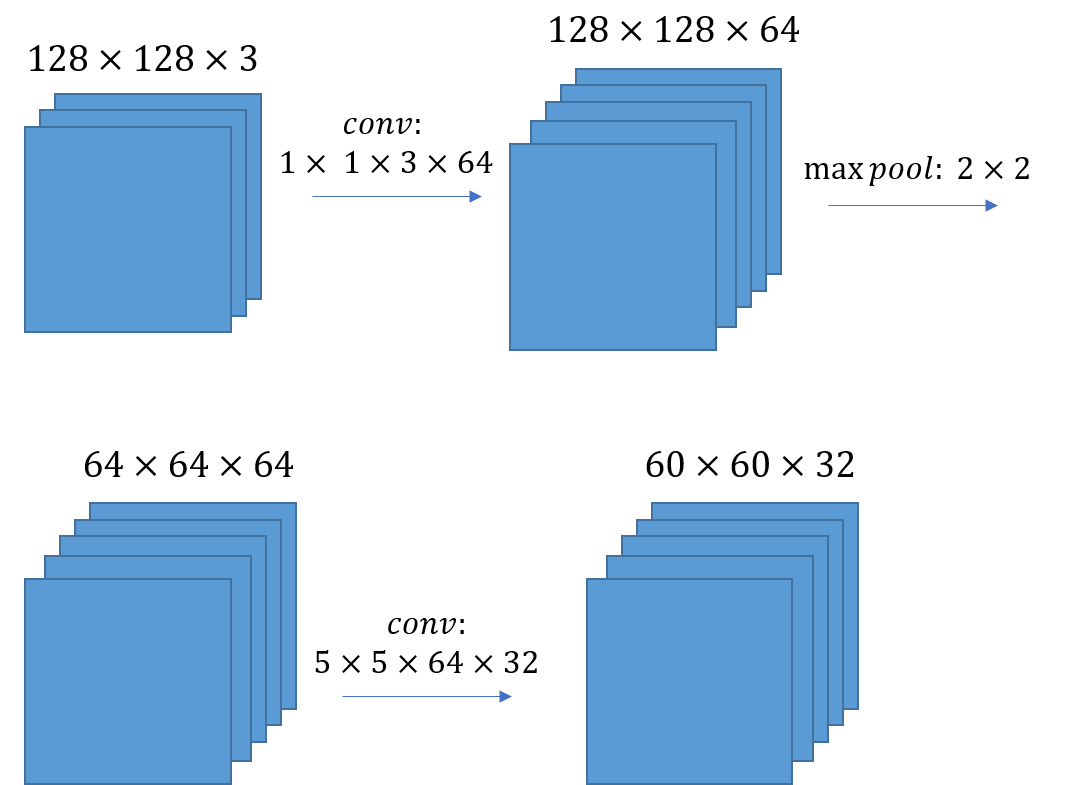
\includegraphics[scale=0.8]{imgs/q_1_1.png}
\newline
\subsubsection{b.}
The convolution of the size 1X1X(?) performs convolution on the same pixes in different channels. The input image contains 3 channels in our case, thus the convolution of the size 1X1X3 fits perfectly to result in a block of new layers without changing size (no need for padding). One kernel results in an output layer of size $128\times128$, but since we have 64 kernels, the depth of the next layers block is 64, accordingly.

\subsubsection{c.}
Let's say, our normalized filter is the following:
\begin{equation*}
\left[
\begin{matrix}
0.1 & 0.2 & 0. 05 \\
0.05 & 0.2 & 0.1 \\
0.15 & 0.1 & 0.05
\end{matrix}
\right]
\end{equation*}

We choose 2 options for stride and padding:

\begin{enumerate}
\item $stride = 2, padding = 1$
The image now has a dimensions of $9\times9$, and with a stride of 1 it gives an output dimensions: $3\times3$
\newline
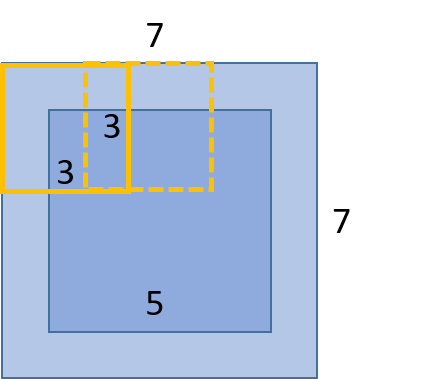
\includegraphics[scale=0.8]{imgs/q_1_31.png}
\newline
Output result is the following:
\item $stride = 1, padding = 2$
The image now has a dimensions of $7\times7$, but with stride of 2 it fits with the filter. Output dimensions: $7\times7$
\newline
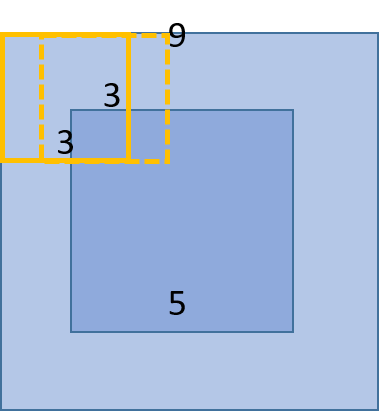
\includegraphics[scale=0.8]{imgs/q_1_32.png}
\newline
Output result is the following:
\end{enumerate}


\end{document}




